\documentclass[../main.tex]{subfiles}

\begin{document}

\section{Az operációs rendszerek alapjai I}

\begin{fulltheorem}
	Az operációs rendszerek alapjai. Az operációs rendszer céljai, feladatai.
	Folyamatok kommunikációja. Termelő-fogyasztó probléma. Postaláda kezelés.
	Szemaforok.
\end{fulltheorem}

\subsection{Az operációs rendszer céljai, feladatai}

Az \kix{operációs rendszer} egy programrendszer, mely közvetítő szerepet
lát el a számítógép felhasználója és a számítógép hardvere között.

Célja a felhasználói programok végrehajtása, felhasználói feladatmegoldás
megkönnyítése, a számítógép rendszer használatának megkönnyítése, a
számítógép hardver kihasználásának hatékonyabbá tétele.

\subsubsection*{Számítógép rendszerek komponense}

\begin{itemize}
	\item \kix{hardver}:
	      az alapvető számítási erőforrásokat nyújtja
	\item \kix{operációs rendszer}:
	      koordinálja és vezérli a hardver erőforrások különböző
	      felhasználók által történő használatát
	\item \kix{alkalmazói programok}:
	      definiáljá azt a módot, ahogyan az egyes rendszererőforrásokat
	      a felhasználók számítási problémáinak megoldásához fel kell használni.
	      (fordítók, adat- bázis kezelők, videó játékok, ügyviteli programok)
	\item \kix{felhasználók}:
	      emberek, gépek, más számítógépek
\end{itemize}

\subsubsection*{Operációs rendszerek komponensei}

\begin{multicols}{2}
	\begin{itemize}
		\item folyamat kezelés
		\item másolagos tár kezelés
		\item fájl kezelés
		\item hálózat-elérés támogatása
		\item memória gazdálkodás
		\item \tc{IO} rendszer kezelés
		\item védelmi rendszer
		\item parancs-interpreter rendszer
	\end{itemize}
\end{multicols}

\subsection{Folyamatok kommunikációja}

A \kix{folyamat} (\cix{process}) egy végrehajtás alatt lévő program.
Bizonyos erőforrásra van szüksége, hogy feladatát megoldhassa.
(\cix{CPU}, memória, állományok, IO berendezések)
Az operációs rendszer az alábbi tevékenységekért felel:
\begin{itemize}
	\item folyamat létrehozása/törlése
	\item folyamat felfüggesztése/újraindítása
	\item eszközök biztosítása
	      (folyamatok szinkronizációjához, kommunikációjához)
\end{itemize}

A folyamat a multiprogramozott operációs rendszerek alapfogalma.
A folyamaton általában műveletek meghatározott sorrendjét értjük.
A folyamat elkezdődik és be is fejeződik.
Minden részművelet végrehajtása csak akkor kezdődhet meg,
ha az előző részművelet végrehajtása már befejeződött.
\begin{itemize}
	\item \kix{független folyamat}:
	      egymás működését semmilyen módon nem befolyásolják

	\item \kix{versengő folyamat}:
	      nem ismerik egymást, de közös erőforráson kell osztozniuk

	\item \kix{együttműködő folyamat}:
	      ismerik egymást, információt cserélnek, együtt dolgoznak
\end{itemize}

Több egymással párhuzamosan futó folyamat gyakran kommunikál közösen használt
memóriaterületek segítségével. Ezek a területek nem érhetőek el egyidejűleg a
folyamatok számára. Az egyidejű hozzáférés kizásása \kix{szemafor}[ok]
segítségével történik.

\subsection{Termelő -- fogyasztó probléma}

Legyen egy \kix{termelő} és egy \kix{fogyasztó} folyamatunk, melyek közös
adatterületet használnak. Ilyenkor fellép a \kix{kölcsönös kizárás} igénye,
hiszen adott memóriaterületet egyszerre csak egy \cix{process} használhat.
Ilyenkor a vezérlés \kix{szemafor} segítségével történik.

\begin{figure}[H]
	\centering
	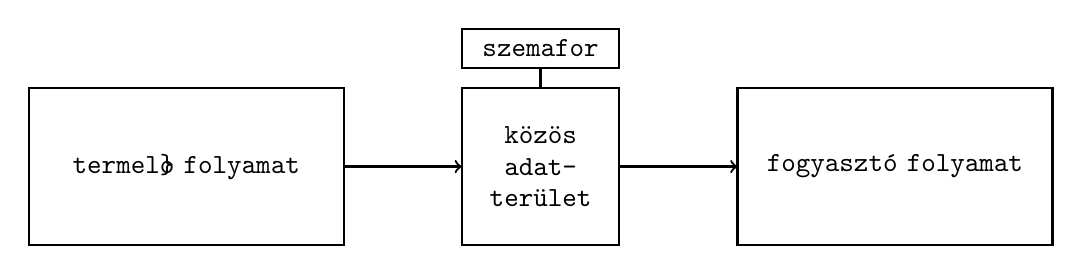
\begin{tikzpicture}
		\draw[thick] (0,0) rectangle ++(4,2);
		\node at (2,1) {\texttt{termelő} \texttt{folyamat}};

		\draw[thick] (5.5,0) rectangle ++(2,2);
		\node at (6.5, 1.4) {\texttt{közös}};
		\node at (6.5, 1) {\texttt{adat-}};
		\node at (6.5, 0.6) {\texttt{terület}};

		\draw[thick] (9,0) rectangle ++(4,2);
		\node at (11,1) {\texttt{fogyasztó} \texttt{folyamat}};

		\draw[thick] (5.5,2.25) rectangle ++(2,.5);
		\node at (6.5,2.5) {\texttt{szemafor}};

		\draw[->, thick] (4,1) -- (5.5,1);
		\draw[->, thick] (7.5,1) -- (9,1);
		\draw[thick] (6.5,2) -- (6.5,2.25);
	\end{tikzpicture}
	\caption{Termelő--fogyasztó probléma}
	\label{fig:semafor}
\end{figure}

Mielőtt a folyamat használni kezdené a közös erőforrást, ellenőriznie kell,
hogy szabad-e. Csak akkor kezdheti el használni, ha a \kix{szemafor} szabadot
jelzett. A primitív megszakíthatatlan, oszthatatlan művelet.
Legyen $P$ (foglalttá állítás) és $V$ (szabaddá állítás) primitívek
$\mathbf{S}$ bináris szemafor.

\begin{figure}[H]
	\centering
	\begin{tikzpicture}
		\draw[
			rounded corners=10,
			color=bgreen,
			ultra thick
		] (0,0) rectangle ++(6,4);
		\draw[
			rounded corners=10,
			color=bgreen,
			ultra thick
		] (7,-1) rectangle ++(7,2);

		\draw[thick, ->] (10, 2.5) to [bend left=20](6,2) {};
		\draw[thick, ->] (6, 1) to [bend right=15](7,0) {};
		\draw[above] node at (10,2.5) {\kix{primitív művelet}};

		\draw node[black, text width=6cm] at (3, 2.25){
			\begin{enumerate}
				\item a szemafor olvasása
				\item beolvasott érték vizsgálata
				\item ha szabad: foglaltra állítás
				\item ha foglalt: vissza 1-re
			\end{enumerate}
		};
		\draw node[black, text width=6cm] at (10.5, 0.25){
			\begin{enumerate}
				\setcounter{enumi}{4}
				\item az erőforrás írása/olvasása
				\item szemafor szabadra áll
			\end{enumerate}
		};
		\draw[below] node at (3,-.5) {
			$P(\mathbf{S})$ $\rightarrow$
			\texttt{memória írás/olvasás}
			$\rightarrow$ $V(\mathbf{S})$
		};
	\end{tikzpicture}
\end{figure}

\subsection{Postaláda kezelés}

A \kix{postaláda} olyan közös adatterület,
ahová egynél több üzenet írható.
Kezelése hasonlít az előző problémához.
A vezérléséhez 3 szemafor szükséges, $P$ és $V$ primitívek:
\begin{itemize}
	\item $\mathbf{S}$ – a kölcsönös kizárást valósítja meg,
	      bináris (\texttt{0-foglalt}, \texttt{1-szabad})

	\item $\mathbf{TELE}$ – a tele helyek száma, nem bináris
	      (értéke: \texttt{0\dots{}N}, kezdetben \texttt{0})

	\item $\text{\textbf{ÜRES}}$ – az üres helyek száma, nem bináris
	      (értéke: \texttt{0\dots{}N}, kezdetben \texttt{N})

	\item $P$ – szemafor értékét eggyel csökkenti (\texttt{foglalttá állítás})

	\item $V$ – szemafor értékét eggyel növeli (\texttt{szabaddá állítás})
\end{itemize}

\begin{figure}[H]
	\centering
	\begin{tikzpicture}
		\draw[thick] (0,0) rectangle ++(4,2);
		\node at (2,1) {\texttt{termelő} \texttt{folyamat}};

		\draw[thick] (5.5,0) rectangle ++(2,2);
		\node at (6.5, 1.4) {\texttt{közös}};
		\node at (6.5, 1) {\texttt{adat-}};
		\node at (6.5, 0.6) {\texttt{terület}};

		\draw[thick] (9,0) rectangle ++(4,2);
		\node at (11,1) {\texttt{fogyasztó} \texttt{folyamat}};

		\draw[thick] (5.5,2.25) rectangle ++(2,.5);
		\node at (6.5,2.5) {\texttt{$\mathbf{S}$}};
		\draw[thick] (6.5,2) -- (6.5,2.25);

		\draw[thick] (6.6,-0.75) rectangle ++(1.8,.5)
		node[midway] {$\text{\textbf{ÜRES}}$};
		\draw[thick] (7,-.25) -- (7,0);

		\draw[thick] (4.6,-0.75) rectangle ++(1.8,.5)
		node[midway] {$\text{\textbf{TELE}}$};
		\draw[thick] (6,-.25) -- (6,0);

		\draw[->, thick] (4,1) -- (5.5,1);
		\draw[->, thick] (7.5,1) -- (9,1);

		\draw[
			rounded corners=10,
			color=bgreen,
			ultra thick
		] (0,-5) rectangle ++(4,4.5)
		node[black, text width=3.5cm, midway]{
				\begin{itemize}
					\item $P(\text{\textbf{ÜRES}})$
					\item $P(\mathbf{S})$
					\item \texttt{mem írás}
					\item $V(\mathbf{S})$
					\item $V(\mathbf{TELE})$
					      \vspace{0.5cm}
				\end{itemize}
			};

		\draw[
			rounded corners=10,
			color=bgreen,
			ultra thick
		] (9,-5) rectangle ++(4,4.5)
		node[black, text width=3.5cm, midway]{
				\begin{itemize}
					\item $P(\mathbf{TELE})$
					\item $P(\mathbf{S})$
					\item \texttt{mem írás}
					\item $V(\mathbf{S})$
					\item $V(\text{\textbf{ÜRES}})$
					      \vspace{0.5cm}
				\end{itemize}
			};
	\end{tikzpicture}
	\caption{Postaláda kezelés}
	\label{fig:mailbox}
\end{figure}

\subsection{Szemaforok}

A közös adatterületet egyszerre csak egy folyamat használhatja.
(\kix{kölcsönös kizárás}) A vezérlés \kix{szemafor}[ok]
segítségével történik. Lehetnek binárisak és nem binárisak.

\end{document}
